\chapter{Attention} \label{chap:attention}

\section{Overview}

A core challenge in Natural Language Processing (NLP) is designing machines capable of understanding human language. Various algorithms have been developed to address this, including recurrent neural networks (RNNs) and more sophisticated architectures like Long Short-Term Memory (LSTM) networks. These models process input tokens sequentially, updating an internal "hidden state" to maintain context. However, because a single hidden state is used to represent all past information, subtle nuances in the language can be lost.

Attention mechanisms offer an alternative approach. Instead of a single hidden state, each token is assigned its own unique representation, and information is selectively passed between these representations. This allows for better preservation of contextual information for future token predictions. Furthermore, the calculations involved in attention mechanisms are highly parallelizable, which enables the training of larger models on more extensive datasets.

% Recurrent neural networks (RNN) and more advanced architectures like Long short-term memory (LSTM) have the ability to \textit{remember} history states while handling the current input token. However, since a single hidden state is shared by all past information, nuances may not be captured precisely. \textbf{Attention} mechanism was developed to address such weaknesses: With attention mechanism, information of tokens are shared between one another, such that each token is exclusively represented by its own hidden state. This means that contextual information is better preserved for future token inferences.

% For example, suppose that we try to capture the meaning of the words \textit{toy car}. Recall that each word is embedded as a vector while being processed, and words with similar meanings are embedded closely. The embedding for \textit{car} should be correlated to vectors associated with \textit{large}, \textit{gasoline-driven} vehicles. With attention mechanism, a contextual embedding is calculated based on the past token \textit{toy}, such that the updated embedding for \textit{car} is no longer correlated to large things but smaller models. In general, attention mechanism can encode much richer information than just a single word in the context, and can determine the relative importance of each component that is attended to.

\section{Attention Mechanism}

Having established that attention mechanisms facilitate information flow between word representations, two key questions emerge:

\begin{enumerate}
    \item From which words should information be retrieved?
    \item What specific information should be transferred?
\end{enumerate}

The answers to these questions form the foundation of attention mechanisms. In the subsequent section, we will begin by exploring the \textbf{single-head attention mechanism}.

\subsection{Single-Head Attention Mechanism}

\begin{figure}
    \centering
    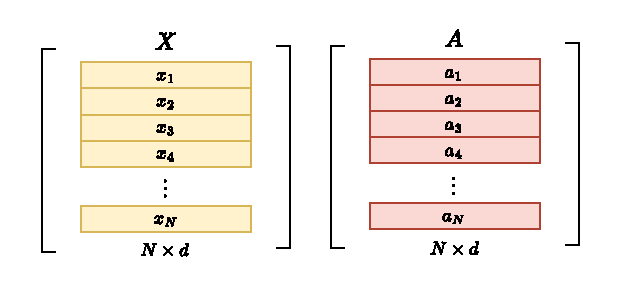
\includegraphics[width=1\linewidth]{fig/X_A.pdf}
    \caption{Left: $N$ input $d$-dimensional vectors stacked into $X$. Right: $N$ attention vectors for each input vector, stacked into $A$. Note that $X$ and $A$ have the same size.}
    \label{fig:X}
\end{figure}

A single-Head attention mechanism operates on sequences of tokens, where a \textbf{token} typically represents a word, sub-word unit, or character. These tokens are transformed into dense vector representations within a $d$-dimensional space, commonly referred to as \textbf{embeddings}. For an input sequence of $N$ tokens, $\{x_i\}_{i=1}^N$, these embeddings are stacked to form an $N \times d$ matrix, denoted as $X$. The goal for single-head attention is to calculate an \textit{attention matrix} $A$ for $X$ such that the $i$-th row of $A$ contains new information for the $i$-th input vector $x_i$: Our understanding of the inputs $X$ is then updated to

$$
X' = X+A.
$$

Figure \ref{fig:X} visualize the input $X$ and the attention matrix $A$.

Intuitively, the calculations for $A$ consists of the following four steps:

\begin{enumerate}
    \item \textbf{Tokens ask}: Who has information for me? (\textit{Query})
    \item \textbf{Tokens reply}: Here is my answer! (\textit{Key})
    \item \textbf{Tokens determine}: I would like to share this piece of information! (\textit{Value})
    \item \textbf{Collect} the pieces of information shared, and \textbf{weight} them according to how well a response answers a query.
\end{enumerate}

To shed more light on the first two steps, consider the below input sequence: \textit{an interesting report} (embedded word-by-word as $(x_1, x_2, x_3)$). Imagine that for the word \textit{report}, it asks: \textit{Any adjectives in front of me?}, and the word \textit{interesting} answers: \textit{I am!}. To capture this question-answering  process mathematically, the question is encoded into a vector $q$ called \textit{query}, via a weight matrix $W^Q$ with size ${d \times d_k}$, where $q_3 = x_3  W^Q.$ Similarly, the answer is encoded in another vector $k_2$ called \textit{key}, via some weight matrix $W^K$ of the same size as $W^Q$, where $k_2 = x_2 W^K$.

To measure how well a key $k_j$ answers a query $q_i$, we compute the dot product between them, i.e., $q_i \cdot k_j$. If two vectors are similar \textit{in direction}, the dot product between them should be relatively large. In this sense, the dot product $q_3 \cdot k_2$ should be large, since $k_2$ is an exact answer to $q_3$. The weight matrices $W^Q$ and $W^K$ are parameters to be trained, such that input vectors can be mapped to good questions and keys that align with the above intuition. In general, the calculations of queries, keys, and determining the similarities of queries and keys, are done in a single matrix multiplication respectively. 
% The computations are illustrated in Figure \ref{fig:XWQ}, \ref{fig:XWK}, and \ref{fig:QK^T}.

% \begin{figure}
%     \centering
%     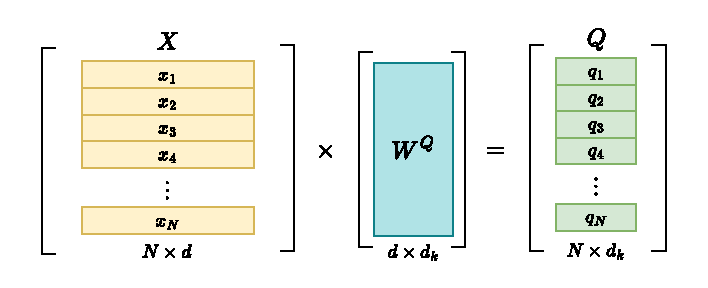
\includegraphics[width=1\linewidth]{fig/XWQ.pdf}
%     \caption{Compute queries $Q$ from input $X$ via weight $W^Q$}.
%     \label{fig:XWQ}
% \end{figure}

% \begin{figure}
%     \centering
%     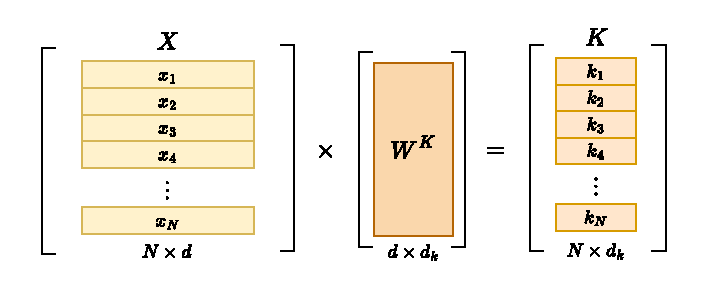
\includegraphics[width=1\linewidth]{fig/XWK.pdf}
%     \caption{Compute keys $K$ from input $X$ via weight $W^K$}
%     \label{fig:XWK}
% \end{figure}

As for the information that a token is to share, it is likewise encoded into a vector $v=xW^V$ called \textit{value}, where $W^V$ is yet another weight matrix with size $d \times d_v$. Since the word \textit{interesting} properly answers the query from \textit{report} (i.e., $q_3 \cdot k_2$ is large), the information passed from \textit{interesting} to \textit{report} should be ``significant'', compared to that passed from \textit{an} to \textit{report}. We capture this ``significance'' of information passed to \textit{report} by regarding  $\{q_3 \cdot k_i\}_{i=1}^4$ as weights, and converting them into a probability distribution via \textit{softmax}: For $i \in \{1, 2, 3, 4\}$, we have $\alpha_{j3} =  \text{softmax}(\{q_3 \cdot k_i\}_i)_j$. The \textit{attention vector} $a_3$ for the word \textit{report} is therefore a weighted sum of $\{v_i\}_{i=1}^4$, where 
$$
a_3 = \sum_{i=1}^{4} \alpha_{i3}v_i.
$$
Repeat this process for all input words, we would obtain the attention matrix $A$! The calculations for \textit{query}, \textit{key} and \textit{value} are illustrated in Figure \ref{fig:XWQ_XWK} and \ref{fig:XWV}, and dot product computations are illustrated in Figure \ref{fig:QK^T}. The single-head attention mechanism can be summarized by a well-known, compact equation:
\begin{equation}\label{eq:1}   
    A = \text{Attention}(Q, K, V) = \text{softmax}\bigg({\frac{QK^T}{\sqrt{d_k}}}\bigg)V, 
\end{equation}
where $\sqrt{d_k}$ is introduced for numerical stability.

\begin{figure}
    \centering
    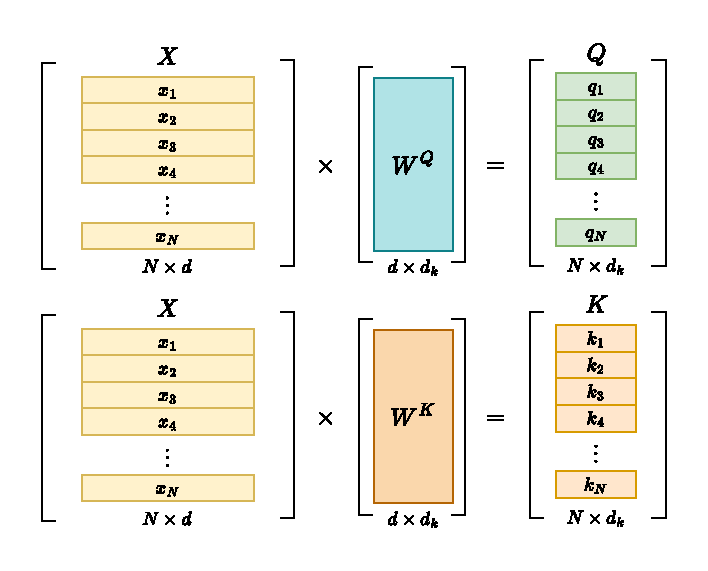
\includegraphics[width=1\linewidth]{fig/XWQ_XWK.pdf}
    \caption{Compute queries $Q$ for input $X$ via weight $W^Q$, and compute keys $K$ for input $X$ via weight $W^K$.}
    \label{fig:XWQ_XWK}
\end{figure}

\begin{figure}
    \centering
    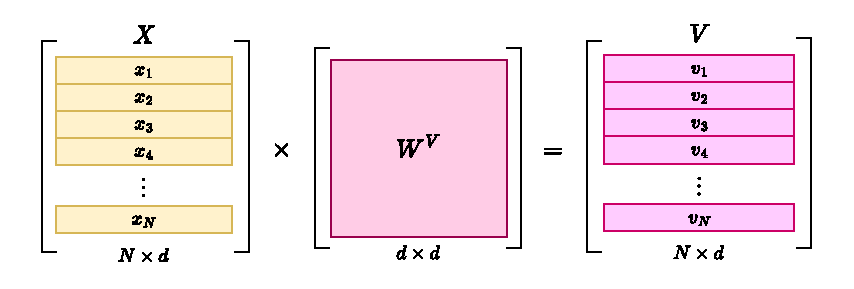
\includegraphics[width=1\linewidth]{fig/XWV.pdf}
    \caption{Compute values $V$ for input $X$ via weight $W^V$. Note that for single-head attention, we must take $d_v = d$ in order for $A$ to match the size of $X$.}
    \label{fig:XWV}
\end{figure}

\begin{figure}
    \centering
    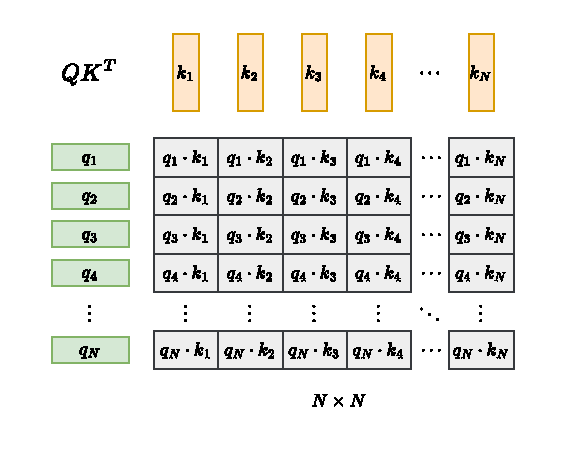
\includegraphics[width=0.8\linewidth]{fig/QK-T.pdf}
    \caption{Compute the similarity (dot product) between all pairs of queries and keys.}
    \label{fig:QK^T}
\end{figure}

\subsection{Multi-Head Attention Mechanism}

A single \textbf{attention head}, as described by Equation \eqref{eq:1}, captures a specific information flow pattern within the context of a sentence. However, natural language exhibits a wide variety of such patterns. Consequently, Transformer models in fact use multi-head attention to combine multiple attention heads. Each head has its own set of weight matrices ($W^Q_i$, $W^K_i$, and $W^V_i$), allowing the input ($X$) to be projected into separate query, key, and value embeddings for each head.

A naive approach to combining $h$ single-head attention outputs would be to sum them: $A = \sum_i A^{(i)}$, where $A^{(i)}$ is the output of $i$-th head. However, this method becomes parameter-inefficient because the weight matrix $W^V_i$, with dimensions $d \times d_v$ (where $d_v = d$ for single-head attention), is substantially larger than $W^Q_i$ and $W^K_i$, both of which have dimensions $d \times d_k$ (where $d_v = d \gg d_k$). This would lead to an unacceptably large number of parameters in the multi-head attention mechanism. To address this, a more parameter-efficient approach was introduced in the original Transformer paper \cite{vaswani2017attention}.

The multi-head attention mechanism refines the process by decomposing the $d \times d$ matrix $W^V_i$ of each head into a product of two smaller matrices: a matrix $W^V_i$ of size $d \times d_v$ and a matrix $W^O_i$ of size $d_v \times d$, where $d_v < d$. While the result of the product has dimensions $d \times d$, this decomposition reduces number of parameters to represent the matrix, but its rank is reduced as well, limiting the fitting power of the model. 

The original Transformer paper maintains the value calculation for each head as $XW^V_i$. With $W^V_i \in \mathbb{R}^{d \times d_v}$, the output of each head has a shape of $N \times d_v$. To obtain an output with dimensions $N \times d$ for the multi-head attention, the outputs from each head (each with dimensions $d \times d_v$) are concatenated horizontally to form a matrix of size $d \times hd_v$. The matrices $W^O_i \in \mathbb{R}^{d_v \times d}$ from each head are then concatenated vertically to produce a matrix $W^O \in \mathbb{R}^{hd_v \times d}$.  Finally, the concatenated head outputs are multiplied by $W^O$ to obtain the final output of the multi-head attention. This process is illustrated in Figure \ref{fig:concat_project_A}.

In summary, multi-head attention enhances the standard attention mechanism by allowing the model to capture multiple different relationships between words in a sentence. It does this by using multiple attention heads with separate weight matrices that project the input into different subspaces, allowing for parallel processing of different aspects of the input. Then, through concatenation and projection the output from each head is combined into a single representation.

% Let $A^{(i)}$ denote the attention matrix calculated from the $i$-th head, and consider there are in total $h$ heads. A naive way to combine all the attention matrices is by summing them up: $A = \sum_i A^{(i)}$. However, a parameter-efficient method is proposed in the original paper \cite{vaswani2017attention}: We concatenate all the attention matrices, resulting in a $N \times hd_v$ matrix, and then apply a transformation $W^O$ of size $hd_v \times d$ on it to map the target matrix back to size $N \times d$ (which matches the size of $X$). This procedure is illustrated in Figure \ref{fig:concat_project_A}. 

% Why this method saves parameters? The naive way takes $p_0 = d \times d$ parameters for $W^V$ in each head (recall that $d_v=d$ for single-head attention). However, for the parameter-efficient method, we can actually choose $d_v < d$ as long as $hd_v > d$. In practice, we have $d_v = d/h$, and thus there is only $d \times d_v = p_0/h$ parameters per $W^V$. As a side note, the dimensions prescribed in the original paper \cite{vaswani2017attention} is: $(d, d_k, d_v, h) = (512, 64, 64, 8)$.

\begin{figure}
    \centering
    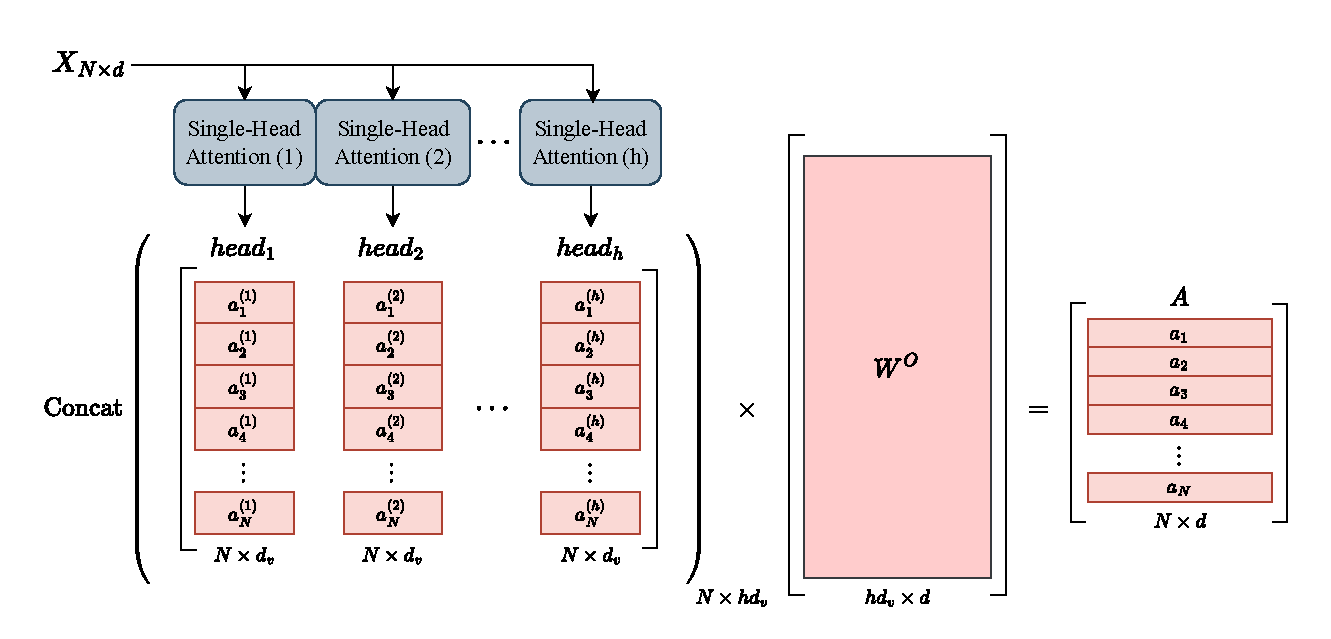
\includegraphics[width=1\linewidth]{fig/concat_project_A.pdf}
    \caption{A parameter-efficient method to accumulate all the attention heads.}
    \label{fig:concat_project_A}
\end{figure}
